\subsection{Running Locally\label{sec:RunningLocally}}
From Visual Studio it is possible to host the team’s EventAPI and Server locally. In order to make the EventAPI contact the local Server, the Solution Configuration must be set to Debug, see Figure \ref{fig:DebugModeScreenshot}. If the configuration is set to Release, the EventAPI will contact the hosted Server instead. \newline
Visual Studio is set up to start an instance of the Server and EventAPI, if they are not running already. The server is now running, and the DCR graph parser or client can be started \\

In some cases our database system cannot automatically create the database. We have provided possible solutions for these problems in Appendix, Section \ref{sec:SolutionsForCreatingTheDatabaseAppendix} \nameref{sec:SolutionsForCreatingTheDatabaseAppendix}

\begin{figure}[h!]
\centering
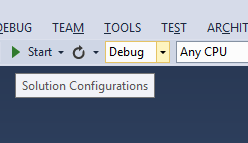
\includegraphics{Figures/SolutionConfigurationsDebug}
\caption{\label{fig:DebugModeScreenshot} Screenshot describing where to set Solution Configuration in Visual Studio}
\end{figure}